%%% CSE 4316 ADS - WORKED EXAMPLE (Full-Stack Web App). Follows ISO/IEC/IEEE 42010:2022 + IEEE 1016-2009.
\documentclass[11pt,letterpaper]{article}
\usepackage[margin=1.0in]{geometry}
\usepackage[T1]{fontenc}\usepackage[bitstream-charter]{mathdesign}\usepackage[latin1]{inputenc}
\usepackage{amsmath}\usepackage{xcolor}\usepackage{cite}\usepackage{hyphenat}
\usepackage{graphicx}\usepackage{float}\usepackage{subfigure}\usepackage{sectsty}
\usepackage[compact]{titlesec}\usepackage[tablegrid]{vhistory}\usepackage{pbox}\usepackage{longtable}
\allsectionsfont{\color{accentcolor}\scshape\selectfont}
\definecolor{accentcolor}{rgb}{0.0,0.0,0.5}
\newcommand{\teamname}{Team Fullstack}
\newcommand{\productname}{CivicPulse Community Service-Request Dashboard}
\newcommand{\coursename}{CSE 4316: Senior Design I}
\newcommand{\semester}{Fall 2026}
\newcommand{\docname}{Architectural Design Specification}
\newcommand{\department}{Department of Computer Science \& Engineering}
\newcommand{\university}{The University of Texas at Arlington}
\newcommand{\authors}{Alan Turing \\ Grace Hopper \\ John Von Neumann \\ Ada Lovelace \\ Charles Babbage}
\usepackage{fancyhdr}\pagestyle{fancy}\usepackage{lastpage}
\lhead{}\chead{}\rhead{}\lfoot{\footnotesize \teamname \ - \semester}\cfoot{}
\rfoot{\footnotesize page \thepage\ of \pageref{LastPage}}
\renewcommand{\headrulewidth}{0.0pt}\renewcommand{\footrulewidth}{0.4pt}
\usepackage[runin]{abstract}\abslabeldelim{\quad}\setlength{\abstitleskip}{-10pt}
\renewcommand{\abstractname}{}\renewcommand{\abstracttextfont}{\color{accentcolor} \small \slshape}

\begin{document}
{\centering \huge \color{accentcolor} \sc \textbf{\department \\ \university} \par}
\vspace{1 in}
{\centering \huge \color{accentcolor} \sc \textbf{\docname \\ \coursename \\ \semester} \par}
\vspace{0.5 in}
\begin{figure}[h!]\centering
\includegraphics[width=0.60\textwidth]{images/test_image}\end{figure}
\vspace{0.5 in}
{\centering \huge \color{accentcolor} \sc \textbf{\teamname \\ \productname} \par}
\vspace{0.5 in}{\centering \large \sc \textbf{\authors} \par}
\newpage
\begin{versionhistory}
  \vhEntry{0.1}{11.02.2026}{JVN}{document creation}
  \vhEntry{1.0}{11.18.2026}{AT|GH|CB}{official release}
\end{versionhistory}
\newpage\setcounter{tocdepth}{2}\tableofcontents\newpage

\section{Introduction}
Architecture of \productname\ as an ISO/IEC/IEEE 42010:2022 \cite{ISO42010}
description using IEEE 1016-2009 \cite{IEEE1016} viewpoints. Refines the SRS.
Scope: the web frontend, backend API, and datastore, plus SSO/geocoding/SMTP
integrations.

\section{Stakeholders \& Architectural Concerns}
\begin{table}[H]\begin{center}\begin{tabular}{ | p{3.5cm} | p{9.5cm} |}\hline
\textbf{Stakeholder} & \textbf{Primary concerns} \\ \hline
City (sponsor) & workflow fit, security, privacy, availability, cost \\ \hline
Residents & easy submission, accessibility, status visibility \\ \hline
Staff agents & efficient triage/assignment, role-appropriate access \\ \hline
City IT & SSO integration, observability, deployability \\ \hline
\end{tabular}\end{center}\end{table}

\section{Architecture Viewpoints}
Context (Section 4), Composition/Data Flow (Section 5), Logical/Functional
(Sections 6--8), Deployment (Section 8). Style: a classic three-tier web
application --- SPA presentation, stateless API, relational + geospatial datastore
--- deployed as containers behind a reverse proxy. Interfaces \texttt{\#NN};
subsystems \texttt{[Layer].[Name]}.

\section{System Overview \& Context View}
\begin{figure}[h!]\centering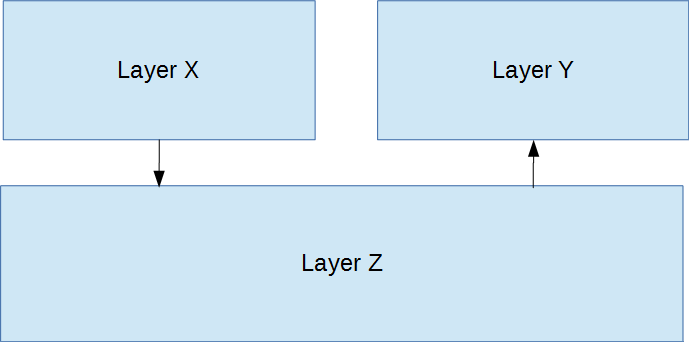
\includegraphics[width=0.55\textwidth]{images/layers}
\caption{Three-tier web architecture}\end{figure}
External actors: residents and staff (browsers), the city SSO (OIDC), the mapping
API, and the SMTP relay. X renders UI; Y enforces logic, auth, and integrations; Z
persists data.

\section{Subsystem Definitions \& Data Flow}
\begin{figure}[h!]\centering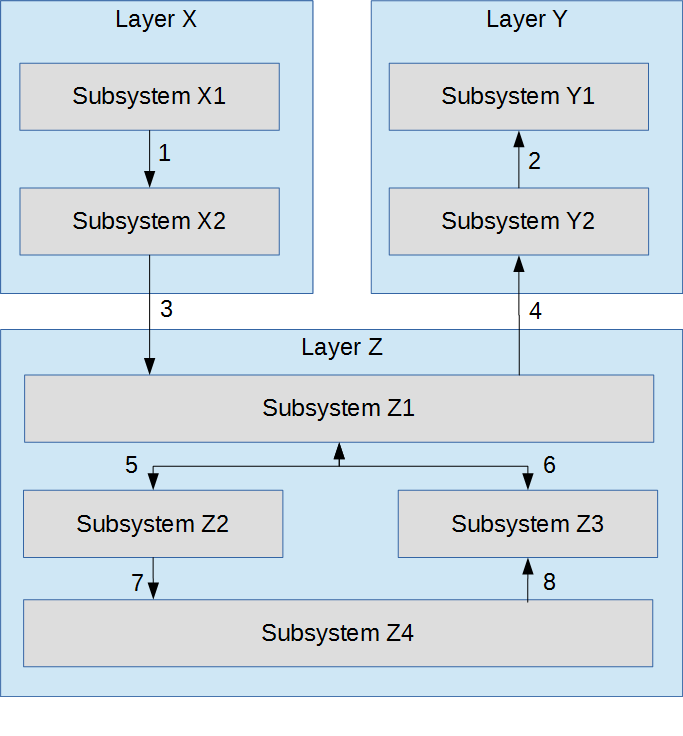
\includegraphics[width=0.9\textwidth]{images/data_flow}
\caption{Browser $\rightarrow$ API $\rightarrow$ services $\rightarrow$ datastore/integrations}\end{figure}

\section{X Layer Subsystems --- Presentation}
\subsection{X.ResidentPortal}
\textbf{Responsibilities:} public SPA for submit/track (FR-01, FR-02), map picker
(EI-02), accessible/responsive (US-01).
\begin{table}[H]\begin{center}\begin{tabular}{ | p{1cm} | p{6cm} | p{2.6cm} | p{2.6cm} |}\hline
ID & Description & Inputs & Outputs \\ \hline
\#01 & Public REST calls & form data & request id, status \\ \hline
\end{tabular}\end{center}\end{table}
\subsection{X.StaffDashboard}
\textbf{Responsibilities:} authenticated SPA for triage/assignment/status (FR-03,
FR-04); RBAC-aware UI (SE-01).

\section{Y Layer Subsystems --- Application}
\subsection{Y.APIGateway}
\textbf{Responsibilities:} single REST entry, TLS termination, OIDC validation, RBAC
enforcement (SE-01).
\begin{table}[H]\begin{center}\begin{tabular}{ | p{1cm} | p{6cm} | p{2.6cm} | p{2.6cm} |}\hline
ID & Description & Inputs & Outputs \\ \hline
\#02 & Authenticated API & requests + token & authorized calls \\ \hline
\end{tabular}\end{center}\end{table}
\subsection{Y.RequestService}
\textbf{Responsibilities:} request lifecycle, triage, assignment, status history
(FR-01--FR-04); duplicate detection (FR-05).
\subsection{Y.NotificationService}
\textbf{Responsibilities:} send status emails via SMTP on status change (FR-04).

\section{Z Layer Subsystems --- Data}
\subsection{Z.Datastore}
\textbf{Responsibilities:} PostgreSQL + PostGIS for requests, users, audit, and
geospatial queries (FR-05 radius). \textbf{Deployment:} managed DB in the cloud
project.
\subsection{Z.ObjectStore}
\textbf{Responsibilities:} store request photos.
\subsection{Z.Integrations}
\textbf{Responsibilities:} adapters for the geocoding API and SMTP relay, isolating
external dependencies behind stable interfaces.

\section{Architecture Decisions \& Rationale}
\subsection{AD-01: Three-tier with stateless API}
\textbf{Context:} multi-role web workflow, need for horizontal scale (PE-01, QA-01).
\textbf{Decision:} stateless API behind a proxy with a shared datastore.
\textbf{Alternatives:} server-rendered monolith (harder to scale/mobile).
\textbf{Consequences:} clean SPA/API split; requires token-based auth. \textbf{Affects:} PE-01, SE-01, QA-01.
\subsection{AD-02: Delegated identity via OIDC}
\textbf{Context:} EI-01/SE-01 --- staff use city credentials. \textbf{Decision:}
delegate to the city IdP; store no staff passwords. \textbf{Alternatives:} local
accounts (more risk, poor fit). \textbf{Consequences:} depends on SSO availability. \textbf{Affects:} EI-01, SE-01.

\section{Requirements Traceability}
\begin{table}[H]\begin{center}\begin{tabular}{ | p{2cm} | p{5.5cm} | p{5cm} |}\hline
\textbf{Req ID} & \textbf{Requirement (abbrev.)} & \textbf{Realizing subsystem(s)} \\ \hline
FR-01/02 & Submit/track & X.ResidentPortal, Y.RequestService \\ \hline
FR-03 & Triage/assign & X.StaffDashboard, Y.RequestService \\ \hline
FR-04 & Status + notify & Y.RequestService, Y.NotificationService \\ \hline
FR-05 & Duplicate detection & Y.RequestService, Z.Datastore \\ \hline
SE-01 & RBAC + TLS & Y.APIGateway \\ \hline
EI-01 & City SSO & Y.APIGateway \\ \hline
\end{tabular}\end{center}\end{table}

\bibliographystyle{reference/IEEEtran_custom}
\bibliography{reference/refs}{}
\end{document}
